%%%%%%%%%%%%%%%%%%%%%%%%%%%%%%%%%%%%%%%%%
% Sullivan Business Report
% LaTeX Template
% Version 1.0 (May 5, 2022)
%
% This template originates from:
% https://www.LaTeXTemplates.com
%
% Author:
% Vel (vel@latextemplates.com)
%
% License:
% CC BY-NC-SA 4.0 (https://creativecommons.org/licenses/by-nc-sa/4.0/)
%
%%%%%%%%%%%%%%%%%%%%%%%%%%%%%%%%%%%%%%%%%

%----------------------------------------------------------------------------------------
%	CLASS, PACKAGES AND OTHER DOCUMENT CONFIGURATIONS
%----------------------------------------------------------------------------------------

\documentclass[
	a4paper, % Paper size, use either a4paper or letterpaper
	12pt, % Default font size, the template is designed to look good at 12pt so it's best not to change this
	%unnumberedsections, % Uncomment for no section numbering
]{include/CSSullivanBusinessReport}

\addbibresource{include/sample.bib} % BibLaTeX bibliography file

%-----------------------------------------------------------------------
%	REPORT INFORMATION
%-----------------------------------------------------------------------
\reporttitle{} % The report title to appear on the title page and page headers, do not create manual new lines here as this will carry over to page headers

\reportsubtitle{A professional layout featuring a large margin\\ and examples of typical business report content} % Report subtitle, include new lines if needed

\reportauthors{Template created by:\\\smallskip Vel (vel@latextemplates.com)} % Report authors/group/department, include new lines if needed

\reportdate{\today} % Report date, include new lines for additional information if needed

\rightheadercontent{
\includegraphics[width=3cm]{./include/creodocs_logo.pdf}} % The content in the right header, you may want to add your own company logo or use your company/department name or leave this command empty for no right header content

\def\tightlist{}
%------------------------------------------------------------------------

\begin{document}

%------------------------------------------------------------------------
%	TITLE PAGE
%------------------------------------------------------------------------
\thispagestyle{empty} % Suppress headers and footers on this page

\begin{fullwidth} % Use the whole page width
	\vspace*{-0.075\textheight} % Pull logo into the top margin
	
	\hfill
\includegraphics[width=5cm]{./include/creodocs_logo.pdf} % Company logo

	\vspace{0.15\textheight} % Vertical whitespace

	\parbox{0.9\fulltextwidth}{\fontsize{50pt}{52pt}\selectfont\raggedright\textbf{\reporttitle}\par} % Report title, intentionally at less than full width for nice wrapping. Adjust the width of the \parbox and the font size as needed for your title to look good.
	
	\vspace{0.03\textheight} % Vertical whitespace
	
	{\LARGE\textit{\textbf{\reportsubtitle}}\par} % Subtitle
	
	\vfill % Vertical whitespace
	
	{\Large\reportauthors\par} % Report authors, group or department
	
	\vfill\vfill\vfill % Vertical whitespace
	
	{\large\reportdate\par} % Report date
\end{fullwidth}

\newpage

%----------------------------------------------------------------------------------------
%	DISCLAIMER/COPYRIGHT PAGE
%----------------------------------------------------------------------------------------
\thispagestyle{empty} % Suppress headers and footers on this page

\begin{twothirdswidth} % Content in this environment to be at two-thirds of the whole page width
	\footnotesize % Reduce font size
	
	\subsection*{Disclaimer}

	Lorem ipsum dolor sit amet, consectetur adipiscing elit. Praesent porttitor arcu luctus, imperdiet urna iaculis, mattis eros. Pellentesque iaculis odio vel nisl ullamcorper, nec faucibus ipsum molestie. Sed dictum nisl non aliquet porttitor. Etiam vulputate arcu dignissim, finibus sem et, viverra nisl. Aenean luctus congue massa, ut laoreet metus ornare in. Nunc fermentum nisi imperdiet lectus tincidunt vestibulum at ac elit.
	
	\subsection*{Copyright}
	
	\textcopyright~[Year] [Company] 
	
	Copyright notice text\ldots In hac habitasse platea dictumst. Curabitur mattis elit sit amet justo luctus vestibulum. In hac habitasse platea dictumst. Pellentesque lobortis justo enim, a condimentum massa tempor eu. Ut quis nulla a quam pretium eleifend nec eu nisl. Nam cursus porttitor eros, sed luctus ligula convallis quis.
	
	\subsection*{Contact}
	
	Address Line 1\\
	Address Line 2\\
	Address Line 3
	
	Business Number 123456
	
	Contact: name@company.com
	
	\vfill % Push the following down to the bottom of the page
	
	\subsubsection*{Changelog}
	
	\scriptsize % Reduce font size further
	
	\begin{tabular}{@{} L{0.05\linewidth} L{0.15\linewidth} L{0.6\linewidth} @{}} % Column widths specified here, change as needed for your content
		\toprule
		v1.0 & 20XX-02-05 & Lorem ipsum dolor sit amet, consectetur adipiscing elit. Praesent porttitor arcu luctus, imperdiet urna iaculis, mattis eros.\\
		v1.1 & 20XX-02-27 & Pellentesque iaculis odio vel nisl ullamcorper, nec faucibus ipsum molestie.\\
		v1.2 & 20XX-03-15 & Sed dictum nisl non aliquet porttitor.\\
		\bottomrule
	\end{tabular}
\end{twothirdswidth}

\newpage

%----------------------------------------------------------------------------------------
%	TABLE OF CONTENTS
%----------------------------------------------------------------------------------------
\begin{twothirdswidth} % Content in this environment to be at two-thirds of the whole page width
	\tableofcontents % Output the table of contents, automatically generated from the section commands used in the document
\end{twothirdswidth}

\newpage

%----------------------------------------------------------------------------------------
%	SECTIONS
%----------------------------------------------------------------------------------------

\section{Situación Actual Sistemas Información SG
(view)}\label{sec:situaciuxf3n-actual-sistemas-informaciuxf3n-sg-view}

\begin{itemize}
\tightlist
\item
  \hyperref[situaciuxf3n-actual.-sistemas-de-informaciuxf3n-sg]{Situación
  Actual. Sistemas de Información SG}

  \begin{itemize}
  \tightlist
  \item
    \hyperref[planteamiento-de-arquitectura-empresarial]{Planteamiento
    de Arquitectura Empresarial}
  \item
    \hyperref[diagnuxf3stico-de-debilidades-tecnoluxf3gicas]{Diagnóstico
    de Debilidades Tecnológicas}
  \item
    \hyperref[brechas-tic-sg]{Brechas TIC SG}
  \item
    \hyperref[1.-introducciuxf3n-y-contexto-estratuxe9gico]{1.
    Introducción y Contexto Estratégico}
  \end{itemize}
\end{itemize}

\newpage

\section{Situación Actual. Sistemas de Información
SG}\label{sec:situaciuxf3n-actual.-sistemas-de-informaciuxf3n-sg}

\subsection{Necesidades y
Aplicaciones}\label{sec:necesidades-y-aplicaciones}

\begin{quote}
\end{quote}

La Secretaría General de la Alcaldía Mayor de Bogotá D.C. está
impulsando un ejercicio de Arquitectura Empresarial (AE) con el
propósito de fortalecer su gestión pública y alcanzar sus objetivos
estratégicos.

\begin{figure}
\centering
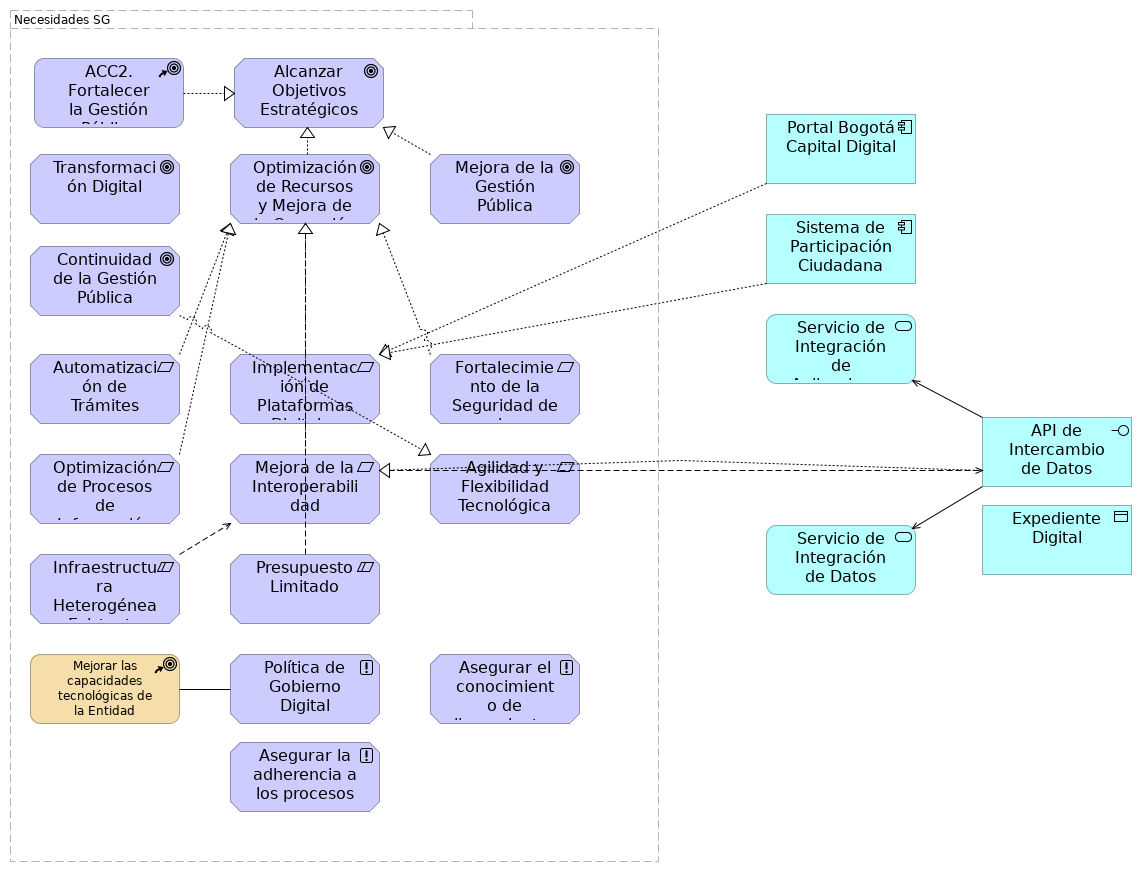
\includegraphics{images/06.3n.NecesidadesyAplicaciones.png}
\caption{06.3n. Necesidades y Aplicaciones. \emph{Fuente: Elaboración
propia con información del equipo servicios tecnológicos de la
OTIC}}\label{fig:id-73084877ba5b4f859a7aa197be93b750}
\end{figure}

\subsubsection{Necesidades SG}\label{sec:necesidades-sg}

\subsubsection{ACC2. Fortalecer la Gestión
Pública}\label{sec:acc2.-fortalecer-la-gestiuxf3n-puxfablica}

Objetivo de TI de alto nivel optimizar (mejorar la eficiencia y
eficacia) los procesos y servicios de la administración pública.

\subsubsection{Alcanzar Objetivos
Estratégicos}\label{sec:alcanzar-objetivos-estratuxe9gicos}

Meta general de la Secretaría General para cumplir con su misión y
visión. \#\#\# Transformación Digital Objetivo clave relacionado con la
modernización y digitalización de los servicios y operaciones.

La transformación digital es un motor fundamental para alinear las
estrategias, procesos y tecnologías de la Secretaría General. Esta
transformación busca:

\begin{itemize}
\tightlist
\item
  Cerrar las brechas en la Política de Gobierno Digital, de la cual la
  Arquitectura Empresarial es un habilitador clave.
\item
  Modernizar la infraestructura tecnológica obsoleta para asegurar su
  continuidad y disponibilidad.
\item
  Integrar plataformas y ecosistemas digitales y superar la falta de
  interoperabilidad.
\item
  Automatizar trámites y estandarizar la gestión y gobernanza de datos
  públicos.
\item
  Adquirir software especializado en análisis de datos para mejorar la
  toma de decisiones basada en evidencia.
\item
  Generar análisis predictivos y prospectivos de resultados de gestión,
  que son insumos para la toma de decisiones.
\item
  Aprovechar nuevas tecnologías como la Inteligencia Artificial para
  mejorar los procesos y la relación con la ciudadanía.
\item
  Fortalecer la ciberseguridad y seguridad de la información para
  proteger la integridad, disponibilidad y confidencialidad de los datos
  y prevenir ataques.
\item
  La disponibilidad de personal adecuado para actualizar plataformas
  tecnológicas es una necesidad identificada para este eje, y los altos
  costos de la tecnología representan una limitación. \#\#\#
  Optimización de Recursos y Mejora de la Operación Objetivo de mejorar
  la eficiencia en el uso de los recursos y la calidad de las
  operaciones internas. \#\#\# Mejora de la Gestión Pública Objetivo
  general de elevar la calidad y el impacto de la gestión gubernamental.
  \#\#\# Continuidad de la Gestión Pública Objetivo de asegurar que los
  programas y proyectos perduren entre diferentes administraciones.
  \#\#\# Automatización de Trámites Necesidad de digitalizar y
  automatizar los procesos de interacción con los ciudadanos. \#\#\#
  Implementación de Plataformas Digitales Requisito para desarrollar o
  adquirir sistemas para trámites y participación ciudadana. \#\#\#
  Fortalecimiento de la Seguridad de la Información Necesidad de
  proteger los datos y sistemas contra amenazas y vulnerabilidades.
  \#\#\# Optimización de Procesos de Información Requisito para mejorar
  la eficiencia y calidad en el manejo de la información. \#\#\# Mejora
  de la Interoperabilidad Necesidad de asegurar la comunicación y el
  intercambio de datos entre diferentes sistemas. \#\#\# Agilidad y
  Flexibilidad Tecnológica Requisito para que las soluciones
  tecnológicas puedan adaptarse rápidamente a nuevos cambios. \#\#\#
  Infraestructura Heterogénea Existente Restricción derivada de la
  diversidad de sistemas y tecnologías ya implementadas. \#\#\#
  Presupuesto Limitado Restricción financiera para la ejecución de
  iniciativas y proyectos. \#\#\# Mejorar las capacidades tecnológicas
  de la Entidad Meta de TI para modernizar y potenciar la
  infraestructura y habilidades tecnológicas. \#\#\# Política de
  Gobierno Digital Principios que guiarán el diseño y la evolución de la
  arquitectura de solución. Son declaraciones de intención de la SG que
  deben ser cumplidas. \#\#\# Asegurar el conocimiento de lineamientos y
  directrices Principios de gobernanza interna. \#\#\# Asegurar la
  adherencia a los procesos y procedimientos establecidos Principios de
  gobernanza interna. \#\#\# Portal Bogotá Capital Digital Plataforma
  unificada creada por la~Secretaría General de la Alcaldía Mayor de
  Bogotá~para facilitar el acceso de la ciudadanía a más de~1.400
  trámites y servicios en línea.
\end{itemize}

\subsubsection{Sistema de Participación
Ciudadana}\label{sec:sistema-de-participaciuxf3n-ciudadana}

Componente de aplicación para facilitar la interacción y el acercamiento
(realimentación) de los ciudadanos.

\subsubsection{Servicio de Integración de
Aplicaciones}\label{sec:servicio-de-integraciuxf3n-de-aplicaciones}

Servicio de aplicación para la unificación y el intercambio de
funcionalidades. \#\#\# API de Intercambio de Datos Interfaz de
aplicación para permitir la comunicación entre diferentes sistemas.
\#\#\# Expediente Digital Objeto de datos en la capa de aplicación que
representa un expediente electrónico. \#\#\# Servicio de Integración de
Datos Servicio de aplicación para la unificación y el intercambio de
información.

\subsection{Diagnóstico de Sistemas de Información SG (análisis de
entorno)}\label{sec:diagnuxf3stico-de-sistemas-de-informaciuxf3n-sg-anuxe1lisis-de-entorno}

\begin{quote}
Arquitectura Empresarial Secretaría General Alcaldía Mayor Bogotá.
Ingenium. 2025 Dominio de Sistemas y Aplicaciones de Software
gestionadas por la OTIC. Sistemas de información del análisis de
entorno.
\end{quote}

Basado en el análisis de las matrices DOFA (Matriz de Evaluación de
Factores Internos - MEFI y Matriz de Evaluación de Factores Externos -
MEFE), se han identificado las siguientes debilidades tecnológicas:

\begin{itemize}
\item
  Sistemas de Información y Datos * Fallas recurrentes en el
  funcionamiento de los sistemas de información y plataformas
  tecnológicas, que afectan la continuidad del servicio y generan
  retrasos y reprocesos. * Insuficiencia en la capacidad de las
  herramientas tecnológicas para la obtención y descarga de material
  probatorio relevante {[}8{]}. * Falta de un software que permita
  extraer información dinámica para la toma de decisiones {[}9{]}. * Se
  realizan análisis descriptivos, pero no predictivos y prospectivos de
  los resultados de la gestión, dificultando la toma de decisiones
  basada en evidencia {[}10{]}. * Cambios en las plataformas
  tecnológicas que no interactúan con las anteriores, generando posibles
  pérdidas de información y reprocesos {[}11{]}.
\item
  Infraestructura Tecnológica * Equipos tecnológicos obsoletos que
  dificultan la ejecución de las actividades {[}12{]}. * Deficiente
  conectividad y falta de interoperabilidad de las plataformas
  tecnológicas {[}13{]}. * Inestabilidad de la conectividad e
  indisponibilidad de servidores de información, comprometiendo la
  operatividad y el cumplimiento de metas {[}14{]}. * Obsolescencia
  tecnológica generalizada que implica la necesidad de renovación de
  equipos y dificulta la prestación de servicios {[}15{]}. * Los altos
  costos de la tecnología pueden limitar la capacidad para implementar y
  mantener sistemas avanzados.
\item
  Seguridad Informática * Vulnerabilidad en la seguridad informática,
  que puede comprometer la integridad de los datos críticos y la
  continuidad operativa. * Vulneración de la inviolabilidad de acceso a
  cuentas de correo institucionales y aplicativos, afectando la reserva
  de la información. * Materialización de riesgos asociados a ataques
  cibernéticos, ingeniería social y suplantación de identidad, poniendo
  en riesgo la seguridad de la información y los documentos (pérdida de
  confidencialidad, integridad y disponibilidad).
\item
  Gestión del Conocimiento y Capacidades Humanas: * Deficiente
  apropiación del conocimiento en procesos de tecnologías de la
  información, generando demora en la solución de servicios. * Falta de
  personal para actualizar las plataformas tecnológicas, lo que genera
  retrasos en la operación.
\item
  Un objetivo clave de la transformación digital es la integración de
  sistemas de información entre entidades públicas y privadas: busca
  mejorar la eficiencia en la operación y el uso de datos de manera
  colaborativa y con calidad.
\item
  La estandarización de procesos y sistemas de información también
  contribuye a la transparencia y rendición de cuentas, fortaleciendo la
  confianza ciudadana en la Gestión Pública.
\item
  El Plan Nacional de Desarrollo ``2022-2026 Colombia, potencia Mundial
  de la vida'' busca fortalecer el Gobierno Digital para una relación
  más eficiente entre el Estado y el ciudadano, utilizando datos y
  tecnologías digitales para mejorar la calidad de vida.
\item
  El Plan Distrital de Desarrollo ``Bogotá Camina Segura 2024-2027''
  también busca incrementar el Índice de Gobierno Digital y elevar el
  Índice de Calidad del Servicio y el Índice de Gestión Pública
  Distrital, con la Arquitectura Empresarial jugando un papel
  habilitador fundamental para la política de Gobierno Digital.
\end{itemize}

Es importante destacar que el proveedor seleccionado deberá realizar la
transferencia de conocimiento sobre el manejo técnico y funcional de la
Herramienta de Arquitectura Empresarial (Repositorio) con la que cuente
la Entidad. Esta herramienta se utilizará para cargar toda la
documentación, modelos, artefactos y demás componentes actualizados
resultantes de los ejercicios de AE.

\begin{figure}
\centering
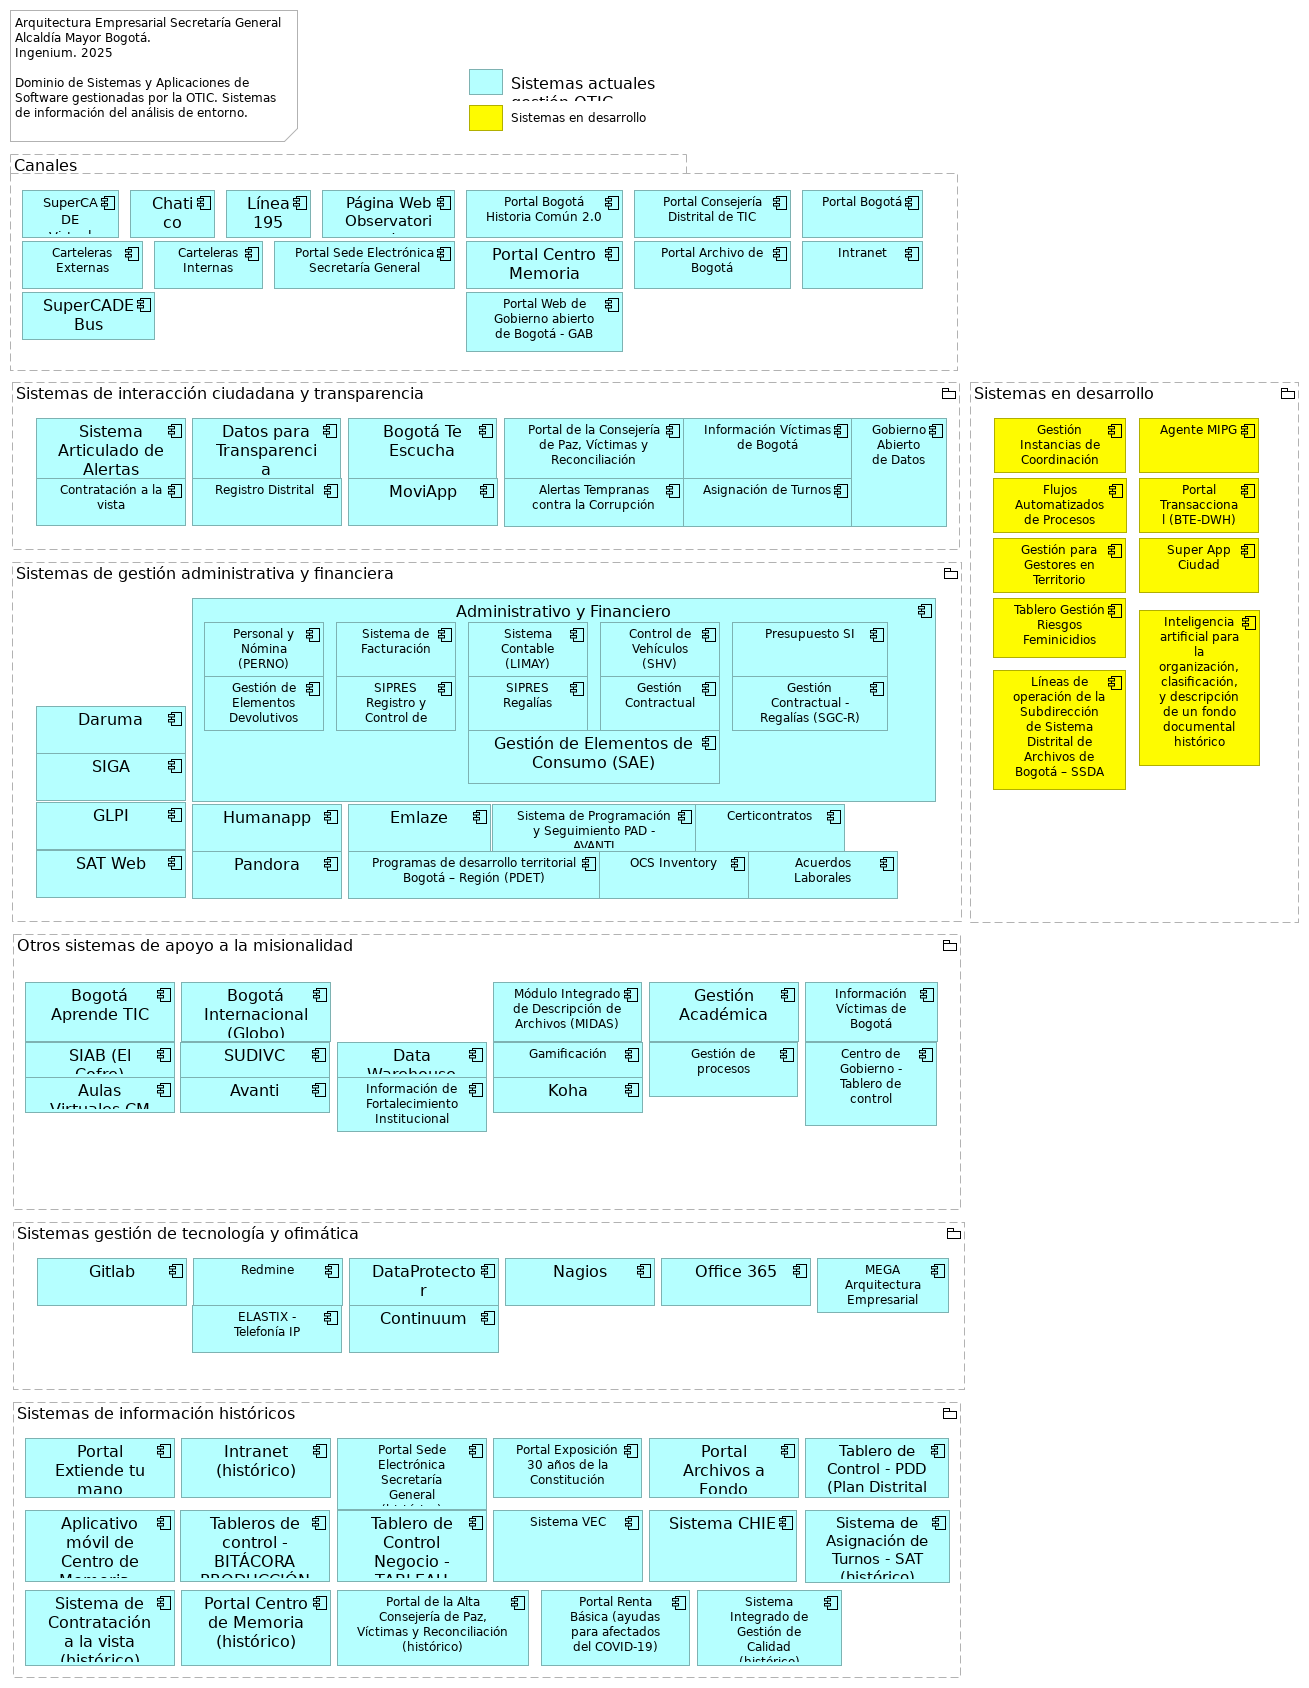
\includegraphics{images/06.2n2.1b.DiagnosticoSI.png}
\caption{06.2n2.1b. Diagnostico SI. \emph{Fuente: Elaboración propia con
información del equipo servicios tecnológicos de la
OTIC}}\label{fig:id-8de5bdda7a914cf9b23955213301db39}
\end{figure}

\subsubsection{Elementos del Modelo}\label{sec:elementos-del-modelo}

\begin{longtable}[]{@{}
  >{\raggedright\arraybackslash}p{(\columnwidth - 4\tabcolsep) * \real{0.3000}}
  >{\raggedright\arraybackslash}p{(\columnwidth - 4\tabcolsep) * \real{0.2000}}
  >{\raggedright\arraybackslash}p{(\columnwidth - 4\tabcolsep) * \real{0.5000}}@{}}
\toprule\noalign{}
\begin{minipage}[b]{\linewidth}\raggedright
Nombre
\end{minipage} & \begin{minipage}[b]{\linewidth}\raggedright
Tipo
\end{minipage} & \begin{minipage}[b]{\linewidth}\raggedright
Documentación
\end{minipage} \\
\midrule\noalign{}
\endhead
\bottomrule\noalign{}
\endlastfoot
Canales & Grouping & \\
SuperCADE Virtual & Application Component & Plataforma digital
desarrollada por la Secretaría General de la Alcaldía Mayor de Bogotá
que permite a la ciudadanía acceder de manera rápida y segura a más de
200 trámites y servicios en línea, sin necesidad de desplazarse
físicamente.~ \\
& & \\
Chatico & Application Component & Agente virtual basado en inteligencia
artificial que facilita el acceso de la ciudadanía a información sobre
trámites, servicios, ayudas distritales y participación ciudadana.
Chatico está disponible a través de la página web oficial y por WhatsApp
(+57 316 0231524). \\
& & \\
Línea 195 & Application Component & Canal telefónico oficial de atención
ciudadana operado por la Secretaría General de la Alcaldía Mayor de
Bogotá. creado para ofrecer información clara, veraz y oportuna sobre
trámites, servicios, campañas y entidades del Distrito Capital. \\
& & \\
Página Web Observatorio de Víctimas del conflicto Armado & Application
Component & Conflicto armado de Bogotá D.C. reportadas por la Oficina
Consejería Distrital de Paz, Victimas y Reconciliacion. \\
& & \\
Portal Bogotá Historia Común 2.0 & Application Component & Portal Bogotá
Historia Común 2.0 es un proyecto de la Secretaría General de la
Alcaldía Mayor de Bogotá, a través del Archivo de Bogotá, que propone
nuevas formas de reconstruir, recuperar y conectar las memorias
barriales y vecinales de la ciudad, brindando acceso libre a los
testimonios, textos, audios, videos y fotografías que forman parte del
patrimonio documental bogotano. La ciudadanía provee historias
cotidianas de su localidad y un grupo de análisis del Archivo de Bogotá
determina la pertinencia para su publicación. \\
\end{longtable}

https://archivobogota.secretariageneral.gov.co/proyectos-estrategicos/bogota-historia-comun/.
\textbar{} \textbar{} Portal Consejería Distrital de TIC \textbar{}
Application Component \textbar{} Portal Alta Consejería Distrital de TIC
de Bogotá donde se publican noticias y eventos relacionados con la
misionalidad de esta dependencia. \textbar{} \textbar{} Portal Bogotá
\textbar{} Application Component \textbar{} Portal de la Alcaldía Mayor
de Bogotá orientado a la publicación de la Gestión del alcalde, noticias
de entidades y noticias de las localidades. \textbar{} \textbar{}
Carteleras Externas \textbar{} Application Component \textbar{} Portales
de visualización pública a la ciudadanía en los sitios de atención. Aquí
se publica la información que aparece en los totems de los Cades.
\textbar{} \textbar{} Carteleras Internas \textbar{} Application
Component \textbar{} Portales de visualización pública a los
funcionarios y contratistas de la Secretaría General. \textbar{}
\textbar{} Portal Sede Electrónica Secretaría General \textbar{}
Application Component \textbar{} Sitio web oficial de la Secretaría
General. Se publica información pública y en cumplimiento de
obligaciones legales, en cumplimiento de la Resolución 1519 de MinTIC.
\textbar{} \textbar{} Portal Centro Memoria \textbar{} Application
Component \textbar{} Herramienta de información para el fomento de la
cultura y los derechos humanos. Publica experiencias vividas para las
víctimas del conflicto armado en Colombia. Sitio
http://centromemoria.gov.co. \textbar{} \textbar{} Portal Archivo de
Bogotá \textbar{} Application Component \textbar{} Portal del Archivo de
Bogotá donde se publican noticias de interes de esta sede. \textbar{}
\textbar{} Intranet \textbar{} Application Component \textbar{} Sistema
web que presta los servicios para actualizar, administrar, monitorear y
optimizar la comunicación interna de la entidad, sirve como instrumento
de divulgación de información vital e importante de la entidad.
\textbar{} \textbar{} SuperCADE Bus Transaccional \textbar{} Application
Component \textbar{} Aplicación de software que permite la
interoperabilidad de los procesos del Distrito, con el fin de realizar
trámites en Línea. Página web que redirige a servicios del Súper CADE.
\textbar{} \textbar{} Portal Web de Gobierno abierto de Bogotá - GAB
\textbar{} Application Component \textbar{} Portal que soporta el
Gobierno Abierto de Bogotá. Cuenta con distintas secciones: datos
destacados de la contratación distrital, datos distritales, datos
abiertos, agendas abiertas, entre otros.
https://gobiernoabiertobogota.gov.co/. \textbar{} \textbar{} Sistemas de
interacción ciudadana y transparencia \textbar{} Grouping \textbar{}
\textbar{} \textbar{} Sistema Articulado de Alertas Tempranas (SAAT)
\textbar{} Application Component \textbar{} Sistema de apoyo a la
estrategia de la Secretaría Distrital de la Mujer (ley Ley 248 de 1995 y
Ley 1257 de 2008): identificación del riesgo posible víctima, gestión
del riesgo y reducción del riesgo. \textbar{} \textbar{} Datos para
Transparencia \textbar{} Application Component \textbar{} Sistema de
tableros de control con datos relevantes, actualizados y comprensibles.
Incluye alertas tempranas contra la corrupción para facilitar la
interacción y el acercamiento (realimentación) de los ciudadanos.
Plataforma que facilita el acceso a datos e información gubernamental.
Soporta al proceso de Gobierno abierto y relacionamiento con la
ciudadanía. https://gobiernoabiertobogota.gov.co/transparencia

\textbar{} \textbar{} Bogotá Te Escucha \textbar{} Application Component
\textbar{} Sistema para el registro de peticiones, quejas y sugerencias
de la ciudadanía \textbar{} \textbar{} Portal de la Consejería de Paz,
Víctimas y Reconciliación \textbar{} Application Component \textbar{}
Portal donde se publican noticias y eventos relacionados con la
misionalidad de la Consejería de Paz, Víctimas y Reconciliación.
\textbar{} \textbar{} Información Víctimas de Bogotá \textbar{}
Application Component \textbar{} Módulo Integrado de Reportes del
Sistema. Sistema de Información de Víctimas de Bogotá - Para registrar
la gestión de atención integral a las víctimas. Sistema que utiliza el
operador externo para realizar entregas de Ayuda Humanitaria Inmediata.
\textbar{} \textbar{} Gobierno Abierto de Datos \textbar{} Application
Component \textbar{} Portal para la publicación de datos abiertos de
Distrito con el fin de ser consultados por la Ciudadanía y utilizados en
toma de decisiones o análisis de información. \textbar{} \textbar{}
Contratación a la vista \textbar{} Application Component \textbar{}
Sistema de registro de contratos distritales \textbar{} \textbar{}
Registro Distrital \textbar{} Application Component \textbar{}
Aplicativo de software para publicar todos los actos administrativos del
Distrito, de cara al ciudadano. \textbar{} \textbar{} MoviApp \textbar{}
Application Component \textbar{} Aplicación móvil para ejercer la
movilidad responsable, a través del uso generalizado de la bicicleta
entre los funcionarios de las diferentes dependencias de la alcaldía.
Aplicativo que permite el uso el registro del uso en bicicleta por parte
de los funcionarios de las entidades del Distrito. \textbar{} \textbar{}
Asignación de Turnos \textbar{} Application Component \textbar{} Sistema
de Asignación de Turnos en los puntos de atención de la ciudad (Cades,
Súper Cades, puntos de encuentro) \textbar{} \textbar{} Sistemas en
desarrollo \textbar{} Grouping \textbar{} \textbar{} \textbar{} Gestión
Instancias de Coordinación \textbar{} Application Component \textbar{}
Aplicación de software para facilitar la interacción y el acercamiento
de los ciudadanos. \textbar{} \textbar{} Agente MIPG \textbar{}
Application Component \textbar{} Agente de inteligencia artificial para
MIPG y temas institucionales de entidades distritales. \textbar{}
\textbar{} Flujos Automatizados de Procesos Empleado con TH y
Contratistas \textbar{} Application Component \textbar{} Flujos
automatizados de procesos de empleado con TH y contratistas para la
gestión de casos ausentismos, permisos comisiones. \textbar{} \textbar{}
Portal Transaccional (BTE-DWH) \textbar{} Application Component
\textbar{} En contratación. Subsecretaria de Servicio a la Ciudadanía.
Diseñar, desarrollar e implementar el portal transaccional de servicio a
la ciudadanía de la Alcaldía Mayor de Bogotá, como el agregador de la
oferta e integración de la demanda de los servicios distritales, que
facilite el acceso ágil y sencillo de la ciudadanía a la oferta
institucional. \textbar{} \textbar{} Gestión para Gestores en Territorio
\textbar{} Application Component \textbar{} Aplicación de software para
recopilación de información de campo de trabajo de gestores
territoriales. \textbar{} \textbar{} Super App Ciudad \textbar{}
Application Component \textbar{} Componente de aplicación para facilitar
la interacción y el acercamiento de los ciudadanos. \textbar{}
\textbar{} Tablero Gestión Riesgos Feminicidios \textbar{} Application
Component \textbar{} Tablero de control para seguimiento de gestión de
riesgos de feminicidios en Bogotá. Proyecto sector Bienestar. \textbar{}
\textbar{} Inteligencia artificial para la organización, clasificación,
y descripción de un fondo documental histórico \textbar{} Application
Component \textbar{} Herramientas de inteligencia artificial para la
organización, clasificación, y descripción del fondo documental
histórico del Archivo General de Bogotá. \textbar{} \textbar{} Líneas de
operación de la Subdirección de Sistema Distrital de Archivos de Bogotá
-- SSDA \textbar{} Application Component \textbar{} En desarrollo.
Aplicación de software para automatización de los procesos de 4 líneas
de operación de la Subdirección de Sistema Distrital de Archivos de
Bogotá - SSDA. \textbar{} \textbar{} Sistemas de gestión administrativa
y financiera \textbar{} Grouping \textbar{} \textbar{} \textbar{}
Administrativo y Financiero \textbar{} Application Component \textbar{}
Grupo de sistema de soporte a la gestión financiera, gestión de
servicios administrativos, tecnológicos, y gestión de recursos físicos.
\textbar{} \textbar{} Personal y Nómina (PERNO) \textbar{} Application
Component \textbar{} Módulo de Personal y Nómina (PERNO, heredado de
SICAPITAL. \textbar{} \textbar{} Sistema de Facturación \textbar{}
Application Component \textbar{} Sistema de Facturación de la
Subdirección de Servicio a la Ciudadanía \textbar{} \textbar{} Sistema
Contable (LIMAY) \textbar{} Application Component \textbar{} LIMAY,
heredado de SICAPITAL. Sistema contable que maneja el libro mayor de la
entidad. \textbar{} \textbar{} Control de Vehículos (SHV) \textbar{}
Application Component \textbar{} Sistema de control de hoja de vida
vehículos. \textbar{} \textbar{} Presupuesto SI \textbar{} Application
Component \textbar{} Sistema presupuestal de la Entidad \textbar{}
\textbar{} Gestión de Elementos Devolutivos (SAI) \textbar{} Application
Component \textbar{} Sistema control de gestión de elementos devolutivos
(SAI, heredado de SICAPITAL). \textbar{} \textbar{} SIPRES Registro y
Control de Presupuesto \textbar{} Application Component \textbar{}
Registro y control de la información de presupuesto de la Secretaría
General (SIPRES). \textbar{} \textbar{} SIPRES Regalías \textbar{}
Application Component \textbar{} Sistema para manejo y control del
presupuesto de regalías (SIPRES REGALIAS). \textbar{} \textbar{} Gestión
Contractual \textbar{} Application Component \textbar{} Sistema de
Gestión Contractual \textbar{} \textbar{} Gestión Contractual - Regalías
(SGC-R) \textbar{} Application Component \textbar{} Sistema de Gestión
Contractual, módulo de regalías \textbar{} \textbar{} Gestión de
Elementos de Consumo (SAE) \textbar{} Application Component \textbar{}
Sistema de control de gestión de elementos de consumo (Heredado
SICAPITAL). \textbar{} \textbar{} Daruma \textbar{} Application
Component \textbar{} Sistema institucional de gestión de la calidad
utilizado por la Secretaría General para centralizar, automatizar y
hacer seguimiento a procesos clave como la administración de documentos,
indicadores, auditorías y acciones de mejora. \textbar{} \textbar{} SIGA
\textbar{} Application Component \textbar{} Sistema Integrado de Gestión
Documental, Archivo y Correspondencia para gestión de todas la
comunicaciones internas de la SG (Memorandos, Circulares, etc), externas
y algunas interoperabilidades. \textbar{} \textbar{} GLPI \textbar{}
Application Component \textbar{} Sistema de soporta a la gestión de
servicios administrativos y tecnológicos, donde se registran y gestionan
las solicitudes de servicios TIC de diferentes categorías de la
Secretaría General. Mesa de ayuda (Gestión de solicitudes de atención
ante incidentes tecnológicos). \textbar{} \textbar{} Humanapp \textbar{}
Application Component \textbar{} Aplicativo de uso interno de la
Secretaría General para generar desprendibles de pago para funcionarios
y certificaciones laborales, de seguridad social y de ingresos y
retenciones. Utiliza una vista del sistema PERNO. Apoya la gestión del
talento humano. Aplicativo de generación de desprendibles de pago para
funcionarios y certificaciones laborales, de seguridad social y de
ingresos y retenciones. \textbar{} \textbar{} Emlaze \textbar{}
Application Component \textbar{} Sistema para la planeación de recursos
empresariales (ERP) de la Imprenta Distrital y control de ejecución y
consumo de insumos en el ejercicio de imprenta. \textbar{} \textbar{}
Sistema de Programación y Seguimiento PAD - AVANTI \textbar{}
Application Component \textbar{} Sistema de Información para registrar
avance de programación y seguimiento de metas plan de desarrollo de la
entidades distritales SDARIV relacionadas con atención integral a las
víctimas. \textbar{} \textbar{} Certicontratos \textbar{} Application
Component \textbar{} Sitio privado interno donde se muestran los
contratos de la entidad, ejecutados desde 2015. \textbar{} \textbar{}
SAT Web \textbar{} Application Component \textbar{} Sistema de
Asignación de Turnos en los puntos de atención a la ciudadanía (Red
Cade). \textbar{} \textbar{} Pandora \textbar{} Application Component
\textbar{} Implementación de temas precontractual y planeación.
\textbar{} \textbar{} Programas de desarrollo territorial Bogotá --
Región (PDET) \textbar{} Application Component \textbar{} Plataforma
tecnológica para habilitar los procesos participativos de construcción
de paz, con énfasis en la formulación de los programas de desarrollo
territorial Bogotá - Región (PDET - BR). \textbar{} \textbar{} OCS
Inventory \textbar{} Application Component \textbar{} Sistema para
gestionar información del inventario de los componentes lógicos de los
elementos ofimáticos \textbar{} \textbar{} Acuerdos Laborales \textbar{}
Application Component \textbar{} Sistema de Información de Acuerdos
Laborales - Registro de los acuerdos laborales entre la SG y los
sindicatos del Distrito \textbar{} \textbar{} Otros sistemas de apoyo a
la misionalidad \textbar{} Grouping \textbar{} \textbar{} \textbar{}
Bogotá Aprende TIC \textbar{} Application Component \textbar{} Portal de
apoya los procesos de Gobierno abierto y relacionamiento con la
ciudadanía, y Fortalecimiento de la Gestión Pública. \textbar{}
\textbar{} Bogotá Internacional (Globo) \textbar{} Application Component
\textbar{} Sistema donde se registran las acciones de Cooperación
Internacional de Bogotá con otras ciudades e instituciones del mundo.
\textbar{} \textbar{} Módulo Integrado de Descripción de Archivos
(MIDAS) \textbar{} Application Component \textbar{} Catalogación y
descripción de algunos registros del Archivo de Bogotá \textbar{}
\textbar{} Gestión Académica \textbar{} Application Component \textbar{}
Moodle para capacitación de servidores de la SG en diferentes temas
\textbar{} \textbar{} Información Víctimas de Bogotá \textbar{}
Application Component \textbar{} Sistema de Información de Víctimas de
Bogotá - Para registrar la gestión de atención integral a las víctimas.
Sistema que utiliza el operador externo para realizar entregas de Ayuda
Humanitaria Inmediata. \textbar{} \textbar{} SIAB (El Cofre) \textbar{}
Application Component \textbar{} Sistema de Información del Archivo de
Bogotá SIAB. Registro del acervo documental de Bogotá (documentos
históricos, planos, mapas, transferencias bibliograficas, entre otros).
Permite automatizar los procesos archivísticos y técnicos que realiza el
Archivo, tales como llevar un registro de los Ingresos Documentales
(antes área de acopio), para la descripción y catalogación de la
documentación, propios del proceso de Gestión de la Función Archivística
y del Patrimonio Documental, para su custodia y conservación permanente.
Utilizado en los procesos de Gobierno abierto y relacionamiento con la
ciudadanía, y Fortalecimiento de la Gestión Pública. \textbar{}
\textbar{} SUDIVC \textbar{} Application Component \textbar{} Sistema
Unificado Distrital de Inspección, Vigilancia y Control - SUDIVC.
\textbar{} \textbar{} Data Warehouse \textbar{} Application Component
\textbar{} Almacenes de datos de trabajo de SG. Bodega de datos con
diversas fuentes de información para el análisis y transformación de
datos de interés. \textbar{} \textbar{} Gamificación \textbar{}
Application Component \textbar{} Herramienta web para el autoaprendizaje
y refuerzo temático para cualificación a servidores públicos \textbar{}
\textbar{} Gestión de procesos \textbar{} Application Component
\textbar{} Sistema de Gestión de procesos \textbar{} \textbar{} Centro
de Gobierno - Tablero de control \textbar{} Application Component
\textbar{} Esta plataforma permite al alcalde y al equipo de gobierno
tener la visión distrital de cada proyecto agilizando la coordinación de
acciones estratégicas encaminadas a la gestión del plan de desarrollo
distrital de Bogotá 2020-2023. \textbar{} \textbar{} Aulas Virtuales CM
\textbar{} Application Component \textbar{} Portal Aulas virtuales del
Centro de Memoria, Paz y Reconciliación. \textbar{} \textbar{} Avanti
\textbar{} Application Component \textbar{} Sistema de Información para
registrar avance de programación y seguimiento de metas plan de
desarrollo de las entidades distritales SDARIV relacionadas con atención
integral a las víctimas. \textbar{} \textbar{} Información de
Fortalecimiento Institucional \textbar{} Application Component
\textbar{} Sistema de Información de Fortalecimiento Institucional
\textbar{} \textbar{} Koha \textbar{} Application Component \textbar{}
Sistema Integrado de Gestión de Bibliotecas. Relacionado con la Gestión
del conocimiento. \textbar{} \textbar{} Sistemas gestión de tecnología y
ofimática \textbar{} Grouping \textbar{} \textbar{} \textbar{} Gitlab
\textbar{} Application Component \textbar{} Plataforma de desarrollo de
software y colaboración. \textbar{} \textbar{} Redmine \textbar{}
Application Component \textbar{} Sistema de documentación técnica de los
Sistemas de Información. Portales Web y Aplicativos de la SG \textbar{}
\textbar{} DataProtector \textbar{} Application Component \textbar{}
Sistema de Copias de seguridad. \textbar{} \textbar{} Nagios \textbar{}
Application Component \textbar{} Sistema de monitoreo de infraestructura
y servicio de TI. \textbar{} \textbar{} Office 365 \textbar{}
Application Component \textbar{} Herramientas de ofimática y
colaboración SG. \textbar{} \textbar{} MEGA Arquitectura Empresarial
\textbar{} Application Component \textbar{} Herramienta de Arquitectura
Empresarial enfocada a los resultados de negocios ayuda a las empresas a
gestionar la innovación e iniciativas estratégicas (también llamado
MEGA). \textbar{} \textbar{} ELASTIX - Telefonía IP \textbar{}
Application Component \textbar{} Aplicación de software para soportar el
servicio de telefonía IP. \textbar{} \textbar{} Continuum \textbar{}
Application Component \textbar{} Herramientas de ofimática y
colaboración SG. Sistema de registro y gestión de uso de las tarjetas de
proximidad de la entidad. \textbar{} \textbar{} Sistemas de información
históricos \textbar{} Grouping \textbar{} \textbar{} \textbar{} Portal
Extiende tu mano \textbar{} Application Component \textbar{} Sistema
donde se gestionan ayudas y se realizan donaciones. \textbar{}
\textbar{} Intranet (histórico) \textbar{} Application Component
\textbar{} Histórico \textbar{} \textbar{} Portal Sede Electrónica
Secretaría General (histórico) \textbar{} Application Component
\textbar{} Histórico. \textbar{} \textbar{} Portal Exposición 30 años de
la Constitución \textbar{} Application Component \textbar{} Portal para
mostrar infografías con motivo del 30º aniversario de la Constitución
Política de Colombia. \textbar{} \textbar{} Portal Archivos a Fondo
\textbar{} Application Component \textbar{} Portal web con motivo de la
celebración del mes del patrimonio para la primera muestra de la
Exposición Archivos a Fondo, con la presentación de veintiún fondos,
colecciones y series documentales, organizada por la Dirección Distrital
de Archivo de Bogotá, de la Secretaría General de la Alcaldía Mayor.
\textbar{} \textbar{} Tablero de Control - PDD (Plan Distrital de
Desarrollo) \textbar{} Application Component \textbar{} Portal web que
visualiza información sobre ejecución, programas metas del PDD.
\textbar{} \textbar{} Aplicativo móvil de Centro de Memoria - CMPR
\textbar{} Application Component \textbar{} Aplicación móvil para las
víctimas del conflicto, busca que los ciudadanos comprendan cómo Bogotá
y sus habitantes han sido afectados por el conflicto armado. \textbar{}
\textbar{} Tableros de control - BITÁCORA PRODUCCIÓN \textbar{}
Application Component \textbar{} Página web de uso privado donde se
publican los tableros de control de uso frecuente del Secretario
General. \textbar{} \textbar{} Tablero de Control Negocio - TABLEAU
Privado \textbar{} Application Component \textbar{} Tablero de Control
Alcalde -Tableau controlado con cinco licencias de uso. Análisis
visuales interactivos que le permite responder a preguntas de negocios
complejas y acceder rápidamente a información que hace crecer su
negocio. Impulsado por nuestra tecnología patentada VizQL, Tableau
proporciona análisis eficaces para hacer preguntas más detalladas y
obtener respuestas más significativas. \textbar{} \textbar{} Sistema VEC
\textbar{} Application Component \textbar{} Sistema donde se registran
actividades de mercados campesinos. \textbar{} \textbar{} Sistema CHIE
\textbar{} Application Component \textbar{} Histórico. Gestión de
acciones y planes de mejora de la Secretaría General (histórico sólo
para consulta). \textbar{} \textbar{} Sistema de Asignación de Turnos -
SAT (histórico) \textbar{} Application Component \textbar{} Sistema de
asignación de turnos para los puntos de atención al ciudadano de la
Secretaría General. \textbar{} \textbar{} Sistema de Contratación a la
vista (histórico) CAV2 \textbar{} Application Component \textbar{}
Histórico. \textbar{} \textbar{} Portal Centro de Memoria (histórico)
\textbar{} Application Component \textbar{} Histórico. \textbar{}
\textbar{} Portal de la Alta Consejería de Paz, Víctimas y
Reconciliación (histórico) \textbar{} Application Component \textbar{}
Histórico. \textbar{} \textbar{} Portal Renta Básica (ayudas para
afectados del COVID-19) \textbar{} Application Component \textbar{}
Sistema de ayudas para los ciudadanos de Bogotá afectados por la
cuarentena del coronavirus (COVID-19). \textbar{} \textbar{} Sistema
Integrado de Gestión de Calidad (histórico) \textbar{} Application
Component \textbar{} Histórico. \textbar{}

Table: Elementos de la vista.
\{\#tbl:tblelement-06.2n2.1b.DiagnosticoSI-id\}

undefined\#\# Planteamiento de Arquitectura Empresarial

La implementación de un ejercicio de Arquitectura Empresarial es clave
para abordar estas debilidades.

\begin{itemize}
\tightlist
\item
  Propósito y Alcance de la AE:

  \begin{itemize}
  \tightlist
  \item
    Comprender la misión, objetivos y metas estratégicas, y definir el
    camino para materializar la visión mediante la alineación de
    estrategias, procesos, talento humano, cultura, información,
    sistemas de información, tecnologías y seguridad {[}18{]}.
  \item
    Incluye un diagnóstico del estado actual (línea base), la definición
    de la arquitectura objetivo (línea destino o meta), el análisis de
    su brecha y la elaboración de una hoja de ruta {[}18, 19{]}.
  \item
    La AE es una práctica estratégica que impulsa las transformaciones
    necesarias para fortalecer la gestión de las entidades y alcanzar
    sus objetivos {[}20{]}.
  \end{itemize}
\item
  Dominios Clave que aborda la AE:

  \begin{itemize}
  \tightlist
  \item
    Arquitectura Institucional: Modelo de capacidades, modelo operativo
    y catálogo de servicios institucionales {[}21{]}.
  \item
    Arquitectura de Información: Definición de flujos y arquitectura de
    información, intercambio de información entre entidades y modelo de
    información institucional, incluyendo la aplicación de Inteligencia
    Artificial.
  \item
    Arquitectura de Sistemas de Información: Definición de arquitecturas
    de referencia para soluciones (SOA), arquitecturas de solución para
    proyectos de SI y caracterización de sistemas de información
    existentes {[}24, 25{]}.
  \item
    Arquitectura de Tecnología: Catálogo de elementos de
    infraestructura, plataforma de interoperabilidad, continuidad y
    disponibilidad de infraestructura, y arquitecturas de referencia
    tecnológica {[}26-28{]}.
  \item
    Arquitectura de Seguridad: Catálogo de servicios de seguridad de la
    información y ciberseguridad, análisis de impacto del negocio,
    arquitectura de seguridad alineada e integrada, y diseño de
    controles de seguridad informática para la gestión de riesgos
    {[}28-30{]}.undefined\#\# Diagnóstico de Debilidades Tecnológicas
  \end{itemize}
\end{itemize}

Con base en el análisis de las matrices DOFA (Matriz de Evaluación de
Factores Internos - MEFI y Matriz de Evaluación de Factores Externos -
MEFE), hemos identificado, y corroborado en el levantamiento de
información de este proyecto, las siguientes debilidades tecnológicas:

\begin{itemize}
\tightlist
\item
  Sistemas de Información y Datos:

  \begin{itemize}
  \tightlist
  \item
    Fallas recurrentes en el funcionamiento de los sistemas de
    información y plataformas tecnológicas, que afectan la continuidad
    del servicio y generan retrasos y reprocesos.
  \item
    Falta de un sistema de información dedicado a la información
    dinámica para la toma de decisiones.
  \item
    Se realizan análisis descriptivos, pero no predictivos y
    prospectivos de los resultados de la gestión, dificultando la toma
    de decisiones basada en evidencia.
  \item
    Cambios en las plataformas tecnológicas que no interactúan con las
    anteriores, con impacto en pérdida de información y reprocesos.
  \end{itemize}
\end{itemize}

undefined\#\# Brechas TIC SG

\begin{itemize}
\tightlist
\item
  Infraestructura Tecnológica:

  \begin{itemize}
  \tightlist
  \item
    Equipos tecnológicos obsoletos que dificultan la ejecución de las
    actividades.
  \item
    Deficiente conectividad y falta de interoperabilidad de las
    plataformas tecnológicas.
  \item
    Inestabilidad de la conectividad e indisponibilidad de servidores de
    información, comprometiendo la operatividad y el cumplimiento de
    metas.
  \item
    Obsolescencia tecnológica generalizada que implica la necesidad de
    renovación de equipos y dificulta la prestación de servicios.
  \item
    Los altos costos de la tecnología pueden limitar la capacidad para
    implementar y mantener sistemas avanzados.
  \end{itemize}
\item
  Seguridad Informática:

  \begin{itemize}
  \tightlist
  \item
    Vulnerabilidad en la seguridad informática, que puede comprometer la
    integridad de los datos críticos y la continuidad operativa.
  \item
    Vulneración de la inviolabilidad de acceso a cuentas de correo
    institucionales y aplicativos, afectando la reserva de la
    información.
  \item
    Materialización de riesgos asociados a ataques cibernéticos,
    ingeniería social y suplantación de identidad, poniendo en riesgo la
    seguridad de la información y los documentos (pérdida de
    confidencialidad, integridad y disponibilidad).
  \end{itemize}
\item
  Gestión del Conocimiento y Capacidades Humanas:

  \begin{itemize}
  \tightlist
  \item
    Deficiente apropiación del conocimiento en procesos de tecnologías
    de la información, generando demora en la solución de servicios.
  \item
    Falta de personal para actualizar las plataformas tecnológicas, lo
    que genera retrasos en la operación. undefined\#\# 1. Introducción y
    Contexto Estratégico
  \end{itemize}
\item
  La Secretaría General de la Alcaldía Mayor de Bogotá D.C. busca
  optimizar su gestión institucional y cumplir sus objetivos
  estratégicos en un entorno dinámico.
\item
  La transformación digital es un pilar fundamental para el desarrollo
  territorial, alineada con el Plan Nacional de Desarrollo 2022--2026 y
  el Plan Distrital de Desarrollo ``Bogotá Camina Segura 2024-2027''.
\item
  El objetivo del ejercicio de Arquitectura Empresarial es fortalecer la
  alineación de sus estrategias, procesos y tecnologías, impulsar la
  transformación digital y promover una gestión pública más eficiente y
  transparente.
\end{itemize}\sidenote{This is a sidenote. This template features a large margin specifically so you can put notes, figures, tables and other things into it as additional material to the main content in the text block.}

Donec in elit ac ante vestibulum rhoncus. Pellentesque ligula tortor, aliquet malesuada nulla tristique vitae. Aliquam mi sem, varius eu pellentesque et, tristique nec quam. Vestibulum pellentesque in dui et venenatis. Sed malesuada elit pellentesque sapien aliquet porta. In at facilisis diam. Duis id ante tellus.\sidenote[][2cm]{This sidenote has been pushed down the page manually with an optional parameter, otherwise it would be right under the one above.} % This first optional argument to a sidenote is the symbol to use (leave this empty for automatic numbering) and the second is the vertical offset (positive is down, negative is up)

In diam libero, vulputate quis accumsan non, auctor in ipsum. Praesent cursus velit eget lacus sodales porta. Proin quis risus ut velit euismod scelerisque ut sed neque. Cras sagittis, dolor ac ullamcorper auctor, tortor dui facilisis diam, at sagittis nisi ipsum a neque. Nullam vel mattis nisi. Ut interdum ut diam at ornare. Nulla ultrices elit justo, vitae tristique massa vulputate sit amet.

\nonumsidenote{
	}Vestibulum erat felis, cursus vitae convallis ac, commodo eu nisi. Nulla facilisi. Mauris dignissim nisi felis, a mollis ex accumsan vel. Suspendisse bibendum vitae nibh in suscipit. Vestibulum et finibus eros. Nulla facilisi. Cras luctus aliquam finibus. In nec justo nec orci malesuada faucibus.

\subsubsection{Subsubsection Title} % Third level section

\begin{fullwidth} % Use the whole page width
	\textit{This is an example of a full width paragraph\ldots} Curabitur id placerat orci. Vivamus pulvinar augue ac feugiat blandit. Donec in ultricies mi. Nam eu lacus ac augue aliquet consectetur. Praesent dui risus, sollicitudin nec felis ut, posuere ultricies dolor. Sed massa nulla, dignissim eget sem sit amet, eleifend fermentum dui. Phasellus consequat sem vel turpis finibus, a aliquam risus malesuada.
\end{fullwidth}

Maecenas consectetur metus at tellus finibus condimentum. Proin arcu lectus, ultrices non tincidunt et, tincidunt ut quam. Integer luctus posuere est, non maximus ante dignissim quis. Nunc a cursus erat. Curabitur suscipit nibh in tincidunt sagittis. Nam malesuada vestibulum quam id gravida. Proin ut dapibus velit. Vestibulum eget quam quis ipsum semper convallis. Duis consectetur nibh ac diam dignissim, id condimentum enim dictum. Nam aliquet ligula eu magna pellentesque, nec sagittis leo lobortis. Aenean tincidunt dignissim egestas. Morbi efficitur risus ante, id tincidunt odio pulvinar vitae.

\paragraph{Paragraph Title} % Fourth level section

Lorem ipsum dolor sit amet, consectetur adipiscing elit. Aliquam auctor mi risus, quis tempor libero hendrerit at. Duis hendrerit placerat quam et semper. Nam ultricies metus vehicula arcu viverra, vel ullamcorper justo elementum. Pellentesque vel mi ac lectus cursus posuere et nec ex.

The section titles below show how multi-line section titles look at the 3 top levels.


%----------------------------------------------------------------------------------------
%	QUOTATIONS
%----------------------------------------------------------------------------------------

\section{Quotations}

Proin mollis urna posuere fringilla. Curabitur finibus, neque vitae vestibulum vestibulum, dolor sapien tincidunt augue, vel porta mauris metus nec mauris. Integer erat magna, porta id erat sed, lacinia volutpat erat. Nulla fermentum tellus arcu, eu iaculis ipsum malesuada aliquam. Duis et lacus maximus, consectetur metus et, eleifend arcu. Vestibulum condimentum diam vitae diam tincidunt viverra.\sidenotequote[-1cm]{\textbf{\LARGE ``}Lorem ipsum dolor sit amet, consectetur adipiscing elit. Praesent porttitor arcu luctus, imperdiet urna iaculis, mattis eros. Pellentesque iaculis odio vel nisl ullamcorper, nec faucibus ipsum molestie.\textbf{''}\\[4pt]\hfill--- John Smith, 1972} % Example margin quotation using the \sidenotequote custom command

\begin{quote}
	\textbf{\LARGE ``}Lorem ipsum dolor sit amet, consectetur adipiscing elit. Praesent porttitor arcu luctus, imperdiet urna iaculis, mattis eros. Pellentesque iaculis odio vel nisl ullamcorper, nec faucibus ipsum molestie. Sed dictum nisl non aliquet porttitor. Etiam vulputate arcu dignissim, finibus sem et, viverra nisl. Aenean luctus congue massa, ut laoreet metus ornare in.\textbf{''}
	
	\hfill--- John Smith, 1972
\end{quote}

Suspendisse tempus odio sit amet volutpat suscipit. Pellentesque ornare libero lacus, non fringilla dolor placerat in. Ut maximus ullamcorper lectus, a pharetra mi sagittis aliquet. Scelerisque augue sed mi fringilla, vel dapibus ligula finibus. Sed ornare velit sem, ac venenatis velit dignissim. Vestibulum ultrices mi at tincidunt condimentum.

%----------------------------------------------------------------------------------------
%	TABLES
%----------------------------------------------------------------------------------------

\section{Table Examples}

This statement automatically references the table below using its label: Table \ref{tab:example}.

%------------------------------------------------

\begin{margintable} % Use the margintable environment for tables to be output to the margin
	\footnotesize % Reduce the font size in the table as space is at a premium
	\caption{Margin table caption.}
	\begin{tabular}{L{0.22\linewidth} C{0.22\linewidth} R{0.25\linewidth}}
		\toprule
		\textbf{Year} & \textbf{Qtr.} & \textbf{Perf.}\\
		\midrule
		20XX & Q1 & 0.5\%\\
		20XX & Q2 & 26.5\%\\
		20XX & Q1 & 35.4\%\\
		20XX & Q4 & 41.3\%\\
		\bottomrule
	\end{tabular}
\end{margintable}

%------------------------------------------------

\begin{table}[H] % [H] forces the table to be output where it is defined in the code (it suppresses floating)
	\caption{Text block table caption.}
	\begin{tabular}{L{0.35\linewidth} L{0.38\linewidth} L{0.16\linewidth}}
		\toprule
		\textbf{Prospect} & \textbf{Industry} & \textbf{Revenue} \\
		\midrule
		Gerlach Inc & Business Development & 3M\\
		Doyle and Sons & Law & 1M\\
		Heathcote Group & Consulting & 12M\\
		Goyette Inc & Advertising & 5M\\
		Holzdeppe GmbH & Manufacturing & 23M\\
		Bienias AG & Accounting & 2.5M\\
		\bottomrule
	\end{tabular}
	\label{tab:example}
\end{table}

%------------------------------------------------

\begin{table*} % Use the table* environment for full width tables
	\caption{Full width table caption.}
	\begin{tabular}{C{0.03\linewidth} L{0.25\linewidth} L{0.27\linewidth} L{0.16\linewidth} L{0.16\linewidth}}
		\toprule
		\textit{\#} & \textbf{Prospect} & \textbf{Industry} & \textbf{Revenue} & \textbf{Employees} \\
		\midrule
		\textit{1} & Gerlach Inc & Business Development & 3M & 65\\
		\textit{2} & Doyle and Sons & Law & 1M & 15\\
		\textit{3} & Heathcote Group & Consulting & 12M & 250\\
		\textit{4} & Goyette Inc & Advertising & 5M & 100\\
		\textit{5} & Holzdeppe GmbH & Manufacturing & 23M & 75\\
		\textit{6} & Bienias AG & Accounting & 2.5M & 40\\
		\bottomrule
	\end{tabular}
\end{table*}

%----------------------------------------------------------------------
%	FIGURES
%----------------------------------------------------------------------

\section{Figure Examples}

This statement automatically references the figure below using its label: Figure \ref{fig:example}.

%------------------------------------------------

\begin{marginfigure} % Use the marginfigure environment for figures to be output to the margin
	
\includegraphics[width=\linewidth]{./include/placeholder.jpg}
	\caption{Margin figure caption.}
\end{marginfigure}

%------------------------------------------------

\begin{figure}[H] % [H] forces the figure to be output where it is defined in the code (it suppresses floating)
	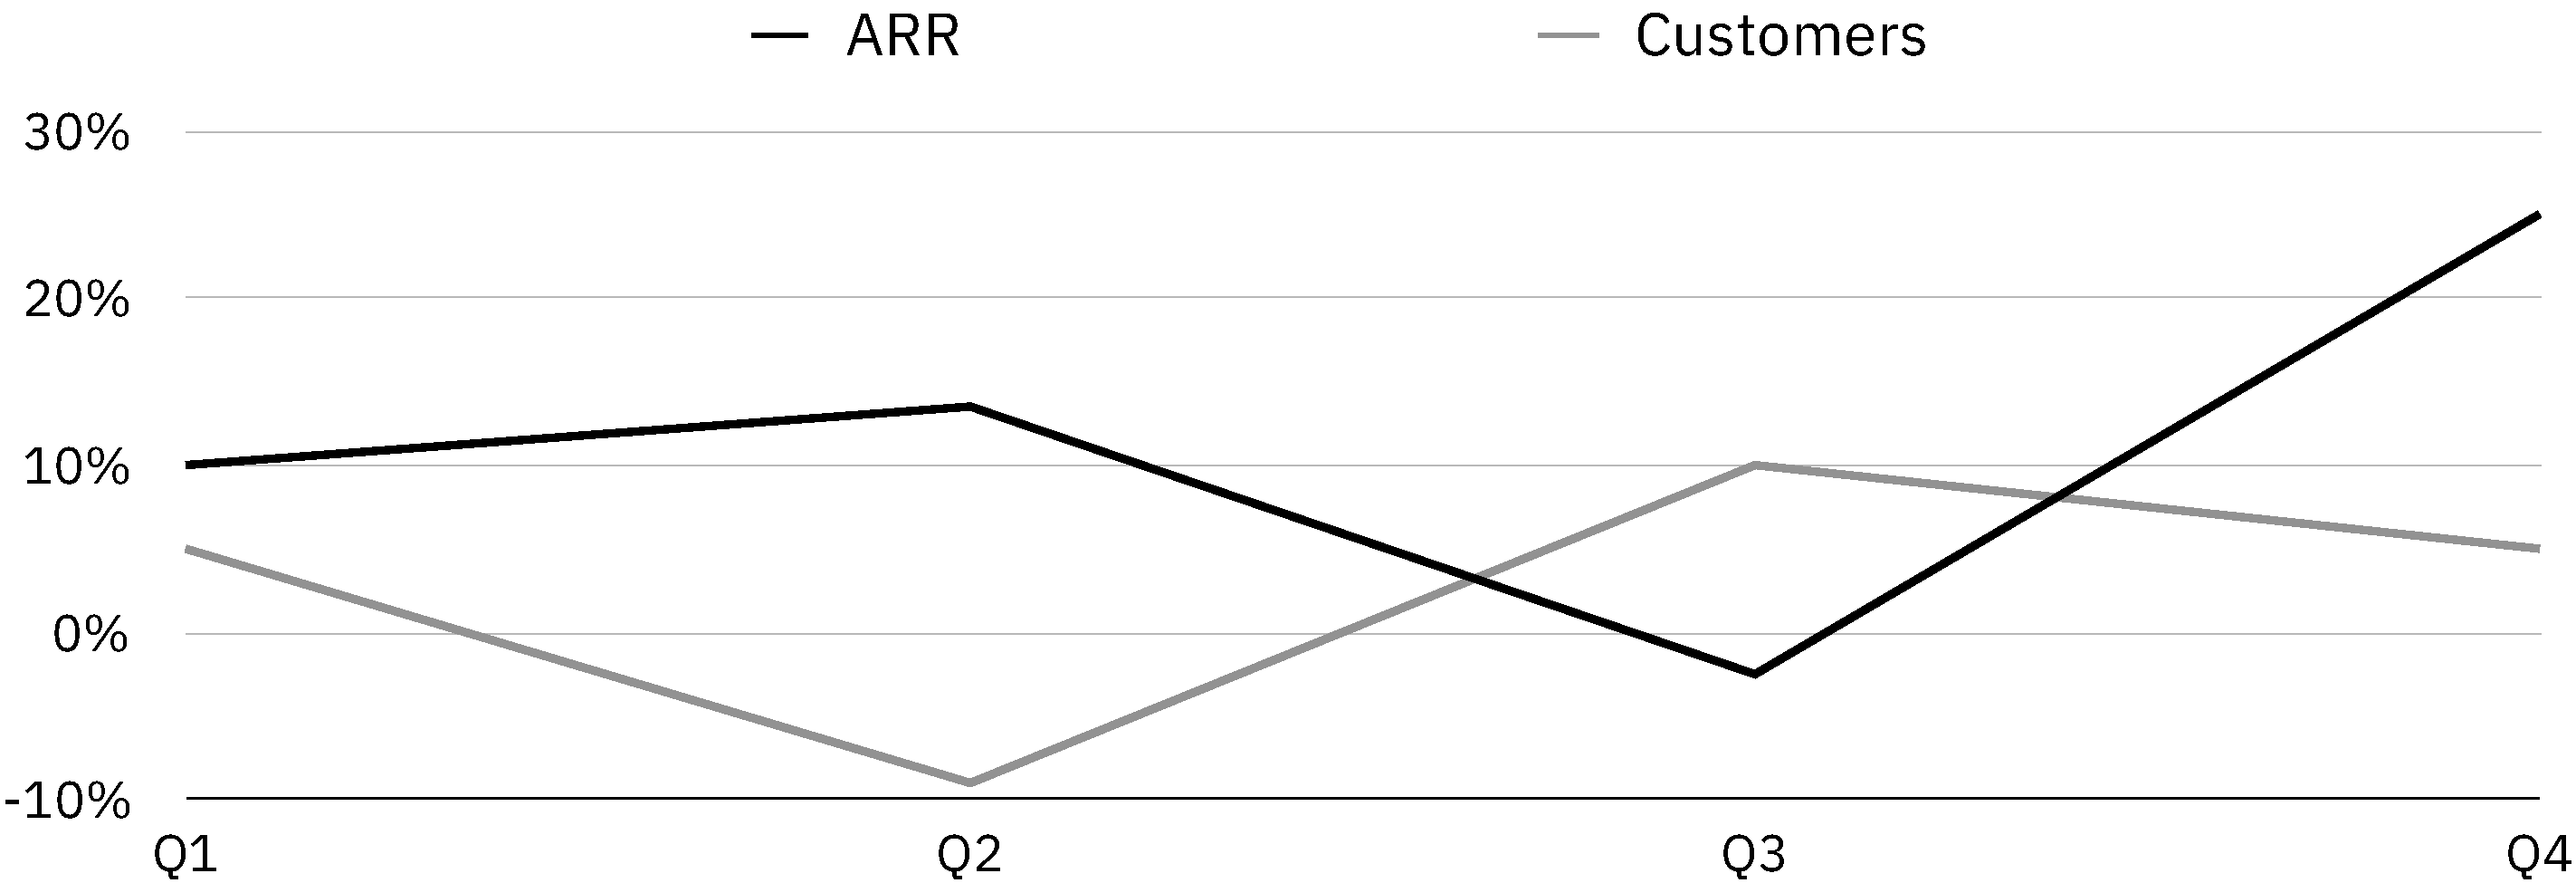
\includegraphics[width=\linewidth]{./include/ARR.pdf}
	\caption{Text block figure caption.}
	\label{fig:example} % Label for referencing this figure in the text automatically
\end{figure}

%------------------------------------------------

\begin{figure*} % Use the figure* environment for full width figures
	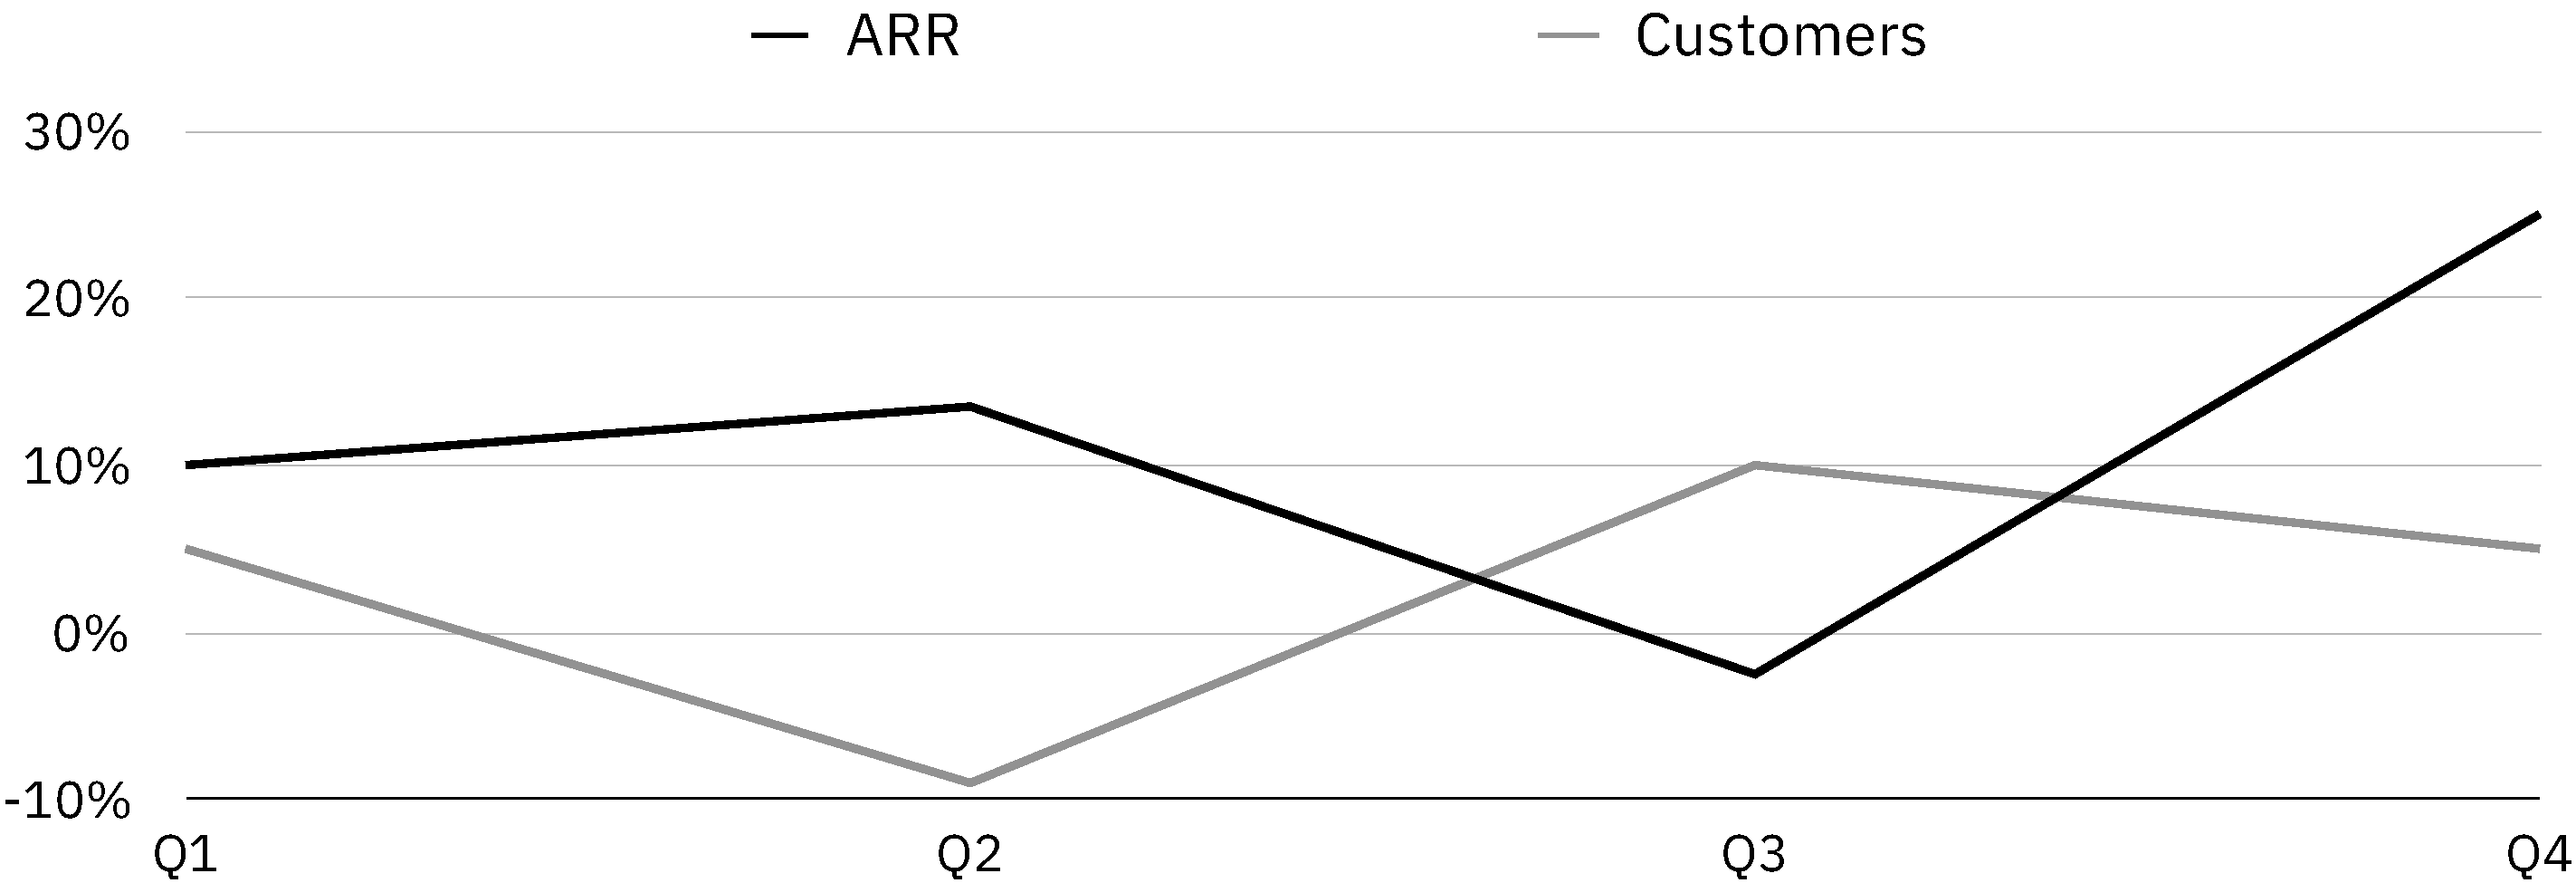
\includegraphics[width=\linewidth]{./include/ARR.pdf}
	\caption{Full width figure caption.}
\end{figure*}

%----------------------------------------------------------------------------------------
%	LISTS
%----------------------------------------------------------------------------------------

\section{List Examples}

\subsection{Bullet Point List}

\nonumsidenote{Bullet point lists can also be created in the margin. For these, we can remove the usual left margin to increase the available horizontal space:\\\medskip \begin{itemize}[leftmargin=*]\item Bullet item one. \item Bullet item two. \item Bullet item three.\end{itemize}}Lorem ipsum dolor sit amet, consectetur adipiscing elit. Praesent porttitor arcu luctus, imperdiet urna iaculis, mattis eros. Pellentesque iaculis odio vel nisl ullamcorper, nec faucibus ipsum molestie. Sed dictum nisl non aliquet porttitor.

\begin{itemize}
	\item First bullet point item
	\begin{itemize}
		\item First indented bullet point item
		\item Second indented bullet point item
		\begin{itemize}
			\item First second-level indented bullet point item
			\item Second second-level indented bullet point item
		\end{itemize}
		\item Third indented bullet point item
	\end{itemize}
	\item Second bullet point item
	\item Third bullet point item
\end{itemize}

Etiam vulputate arcu dignissim, finibus sem et, viverra nisl. Aenean luctus congue massa, ut laoreet metus ornare in. Nunc fermentum nisi imperdiet lectus tincidunt vestibulum at ac elit. Nulla mattis nisl eu malesuada suscipit.

%------------------------------------------------

\subsection{Numbered List}

\nonumsidenote[-2.5cm]{Numbered lists can also be created in the margin. For these, we can remove the usual left margin to increase the available horizontal space:\\\medskip \begin{enumerate}[leftmargin=*]\item Numbered item one. \item Numbered item two. \item Numbered item three.\end{enumerate}}Lorem ipsum dolor sit amet, consectetur adipiscing elit. Praesent porttitor arcu luctus, imperdiet urna iaculis, mattis eros. Pellentesque iaculis odio vel nisl ullamcorper, nec faucibus ipsum molestie. Sed dictum nisl non aliquet porttitor.

\begin{enumerate}
	\item First numbered item
	\begin{enumerate}
		\item First indented numbered item
		\item Second indented numbered item
		\begin{enumerate}
			\item First second-level indented numbered item
			\item Second second-level indented numbered item
		\end{enumerate}
		\item Third indented numbered item
	\end{enumerate}
	\item Second numbered item
	\item Third numbered item
\end{enumerate}

Etiam vulputate arcu dignissim, finibus sem et, viverra nisl. Aenean luctus congue massa, ut laoreet metus ornare in. Nunc fermentum nisi imperdiet lectus tincidunt vestibulum at ac elit. Nulla mattis nisl eu malesuada suscipit.

%------------------------------------------------

\subsection{Description List}

\nonumsidenote{Description lists can also be created in the margin:\\\medskip \begin{description}\item[A1] Description item one. \item[B1] Description item two. \item[C1] Description item three.\end{description}}Lorem ipsum dolor sit amet, consectetur adipiscing elit. Praesent porttitor arcu luctus, imperdiet urna iaculis, mattis eros. Pellentesque iaculis odio vel nisl ullamcorper, nec faucibus ipsum molestie. Sed dictum nisl non aliquet porttitor.

\begin{description}
	\item[Item One] Lorem ipsum dolor sit amet, consectetur adipiscing elit. Praesent porttitor arcu luctus, imperdiet urna iaculis, mattis eros. Pellentesque iaculis odio vel nisl ullamcorper, nec faucibus ipsum molestie.
	\item[Item Two] Sed dictum nisl non aliquet porttitor.
	\begin{description}
		\item[Subitem] Maecenas consectetur metus at tellus finibus condimentum. Proin arcu lectus, ultrices non tincidunt et, tincidunt ut quam. Integer luctus posuere est, non maximus ante dignissim quis.
		\begin{description}
			\item[Subsubitem] Maecenas consectetur metus at tellus finibus condimentum. Proin arcu lectus, ultrices non tincidunt et, tincidunt ut quam. Integer luctus posuere est, non maximus ante dignissim quis.
	\end{description}
	\end{description}
	\item[Item Three] Etiam vulputate arcu dignissim, finibus sem et, viverra nisl. Aenean luctus congue massa, ut laoreet metus ornare in. Nunc fermentum nisi imperdiet lectus tincidunt vestibulum at ac elit. Nulla mattis nisl eu malesuada suscipit.
\end{description}

Etiam vulputate arcu dignissim, finibus sem et, viverra nisl. Aenean luctus congue massa, ut laoreet metus ornare in.

%----------------------------------------------------------------------------------------
%	REFERENCING CITATIONS
%----------------------------------------------------------------------------------------

\section{Referencing Citations}

This statement requires citation \autocite{Smith:2024jd}.

This statement requires multiple citations \autocite{Smith:2024jd, Smith:2023qr}.

This short citation is in the margin\sidecite{Smith:2023qr}.

This long citation is in the margin\fullsidecite{Smith:2024jd}.

This statement has an in-text citation: \textcite{Smith:2024jd}.

%----------------------------------------------------------------------------------------
%	LINKS
%----------------------------------------------------------------------------------------

\section{Link Examples}

This is a URL link: \href{https://www.duckduckgo.com}{DuckDuckGo}.\nonumsidenote{Links can be clicked in the PDF to navigate to the linked website or email address.}

This is a email link: \href{mailto:example@example.com}{example@example.com}.

This is a monospaced URL link: \url{https://duckduckgo.com}.


%----------------------------------------------------------------------------------------
%	CODE
%----------------------------------------------------------------------------------------

\section{Displaying Code}

The block below is a code listing. It displays code in an easy to use way with line numbers for quick reference to specific parts of the code.

\begin{lstlisting}
{
	"city": [
		{
			"id": 1,
			"name": "Toronto",
			"country": "Canada",
			"population": 6200000
		},
		{
			"id": 2,
			"name": "New York",
			"country": "United States of America",
			"population": 8800000
		}
	]
}
\end{lstlisting}

%----------------------------------------------------------------------------------------
%	 REFERENCES/BIBLIOGRAPHY
%----------------------------------------------------------------------------------------

\newpage

\addcontentsline{toc}{section}{Reference List} % Add the bibliography to the table of contents

\begin{twothirdswidth} % Content in this environment to be at two-thirds of the whole page width
	\printbibliography[title=Reference List] % Output the bibliography with a custom section title
\end{twothirdswidth}

%----------------------------------------------------------------------------------------
%	APPENDICES
%----------------------------------------------------------------------------------------

\newpage

\section*{Appendices}

\begin{appendices}

\section{Appendix Section}

Lorem ipsum dolor sit amet, consectetur adipiscing elit. Aliquam auctor mi risus, quis tempor libero hendrerit at. Duis hendrerit placerat quam et semper. Nam ultricies metus vehicula arcu viverra, vel ullamcorper justo elementum. Pellentesque vel mi ac lectus cursus posuere et nec ex. Fusce quis mauris egestas lacus commodo venenatis. Ut at arcu lectus. Donec et urna nunc. Morbi eu nisl cursus sapien eleifend tincidunt quis quis est. Donec ut orci ex. Praesent ligula enim, ullamcorper non lorem a, ultrices volutpat dolor. Nullam at imperdiet urna. Pellentesque nec velit eget euismod pretium.

\section{Appendix Section}

Lorem ipsum dolor sit amet, consectetur adipiscing elit. Aliquam auctor mi risus, quis tempor libero hendrerit at. Duis hendrerit placerat quam et semper. Nam ultricies metus vehicula arcu viverra, vel ullamcorper justo elementum. Pellentesque vel mi ac lectus cursus posuere et nec ex. Fusce quis mauris egestas lacus commodo venenatis. Ut at arcu lectus. Donec et urna nunc. Morbi eu nisl cursus sapien eleifend tincidunt quis quis est. Donec ut orci ex. Praesent ligula enim, ullamcorper non lorem a, ultrices volutpat dolor. Nullam at imperdiet urna. Pellentesque nec velit eget euismod pretium.

\section{Appendix Section}

Lorem ipsum dolor sit amet, consectetur adipiscing elit. Aliquam auctor mi risus, quis tempor libero hendrerit at. Duis hendrerit placerat quam et semper. Nam ultricies metus vehicula arcu viverra, vel ullamcorper justo elementum. Pellentesque vel mi ac lectus cursus posuere et nec ex. Fusce quis mauris egestas lacus commodo venenatis. Ut at arcu lectus. Donec et urna nunc. Morbi eu nisl cursus sapien eleifend tincidunt quis quis est. Donec ut orci ex. Praesent ligula enim, ullamcorper non lorem a, ultrices volutpat dolor. Nullam at imperdiet urna. Pellentesque nec velit eget euismod pretium.

\end{appendices}

%----------------------------------------------------------------------------------------

\end{document}
